\documentclass[10pt,a4paper]{beamer}
\usetheme{Szeged}
\usecolortheme{beaver}

\usepackage[utf8]{inputenc}
\usepackage{amsmath}
\usepackage{amsfonts}
\usepackage{amssymb}
\usepackage{inputenc}
\usepackage[lined,boxed,ruled,commentsnumbered]{algorithm2e}



\title % (optional, only for long titles)
{Análise de \textit{Timing} Estática e a Avaliação do Impacto do Atraso das Interconexões em Circuitos Digitais}
\author % (optional, for multiple authors)
{Chrystian de Sousa Guth}
\institute[UFSC] % (optional)
{
  Curso de Bacharelado em Ciências da Computação\\
  Universidade Federal de Santa Catarina

}
\date[nov12] % (optional)
{Novembro de 2013}
\subject{Computação}


\begin{document}

	% CAPA
	\frame{\titlepage}
	
	% SUMARIO
	\begin{frame}
		\frametitle{Sumário}
		\tableofcontents[]
	\end{frame}

	\section{Introdução}
		
		\subsection*{}
			\begin{frame}
				\frametitle{Fluxo \textit{Standard Cell}}
				olá
			\end{frame}
		
			\begin{frame}
				\frametitle{Motivação}
				olá
			\end{frame}
		
			\begin{frame}
				\frametitle{Justificativa}
				olá
			\end{frame}
		
			\begin{frame}
				\frametitle{Objetivos}
				olá
			\end{frame}
			
			\begin{frame}
				\frametitle{Escopo}
				olá
			\end{frame}
		
	
	\section{Conceitos}
		
		\begin{frame}
		\frametitle{Características Temporais dos Circuitos Digitais}
			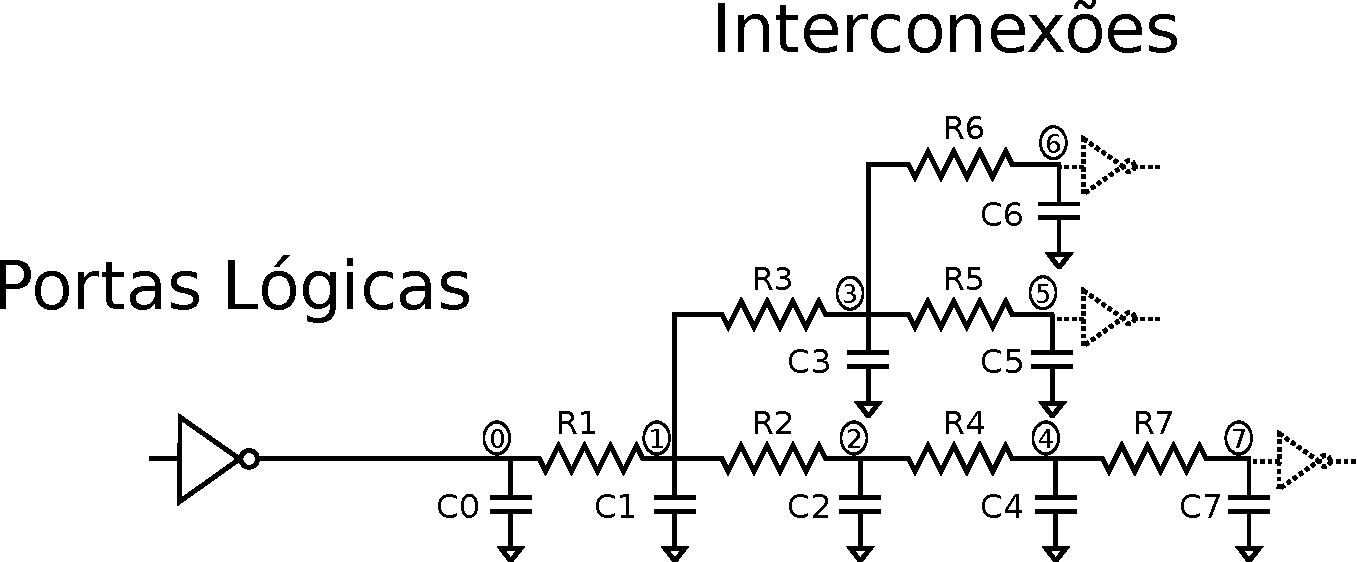
\includegraphics[width=\textwidth]{img/circuito.pdf} 
		\end{frame}

		\subsection*{Portas Lógicas}
			\begin{frame}
				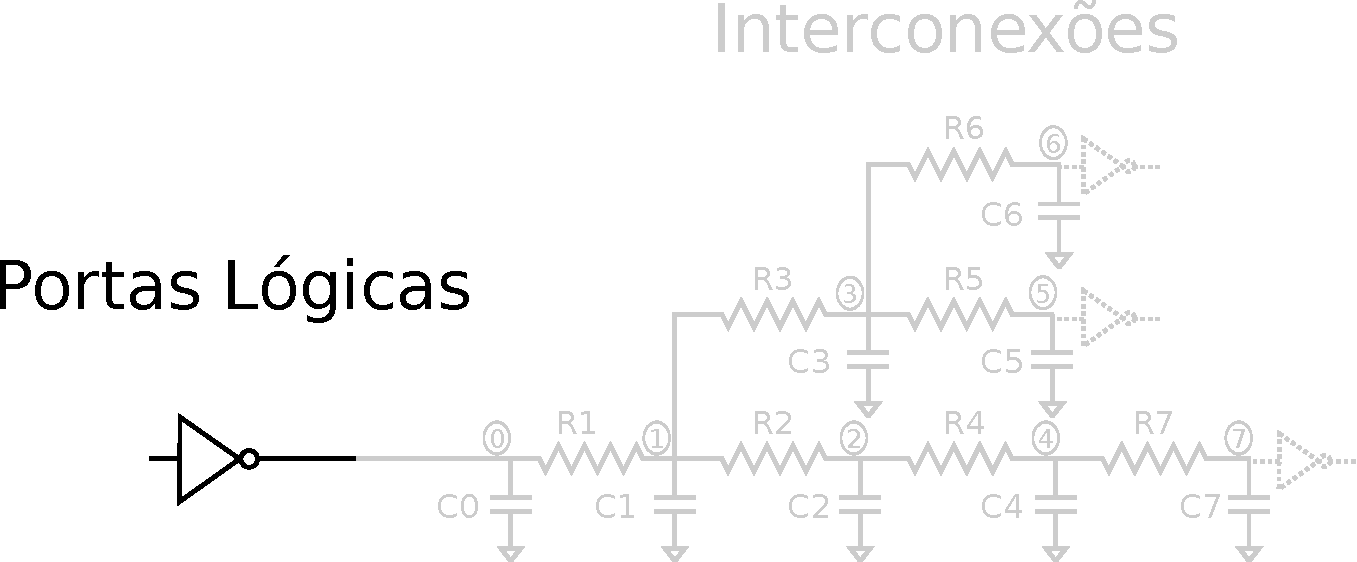
\includegraphics[width=\textwidth]{img/circuito_portas.pdf} 
			\end{frame}
			
			\begin{frame}
				\frametitle{Características Temporais}
				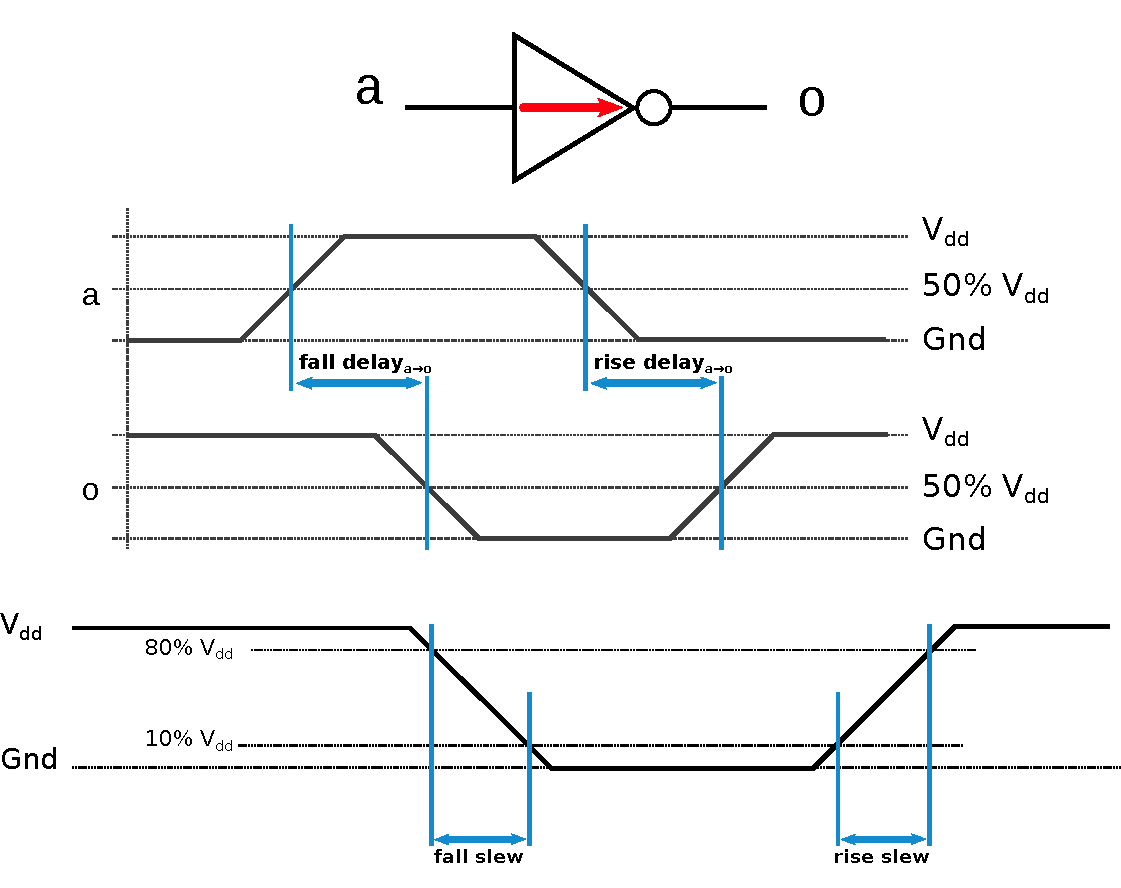
\includegraphics[width=0.8 \textwidth]{img/caracteristicas_temporais_portas_logicas.pdf} 
			\end{frame}
			
			\begin{frame}
				\frametitle{Modelo de Atraso Não-Linear}
			\end{frame}
		
		\subsection*{Interconexões}

			
			\begin{frame}
				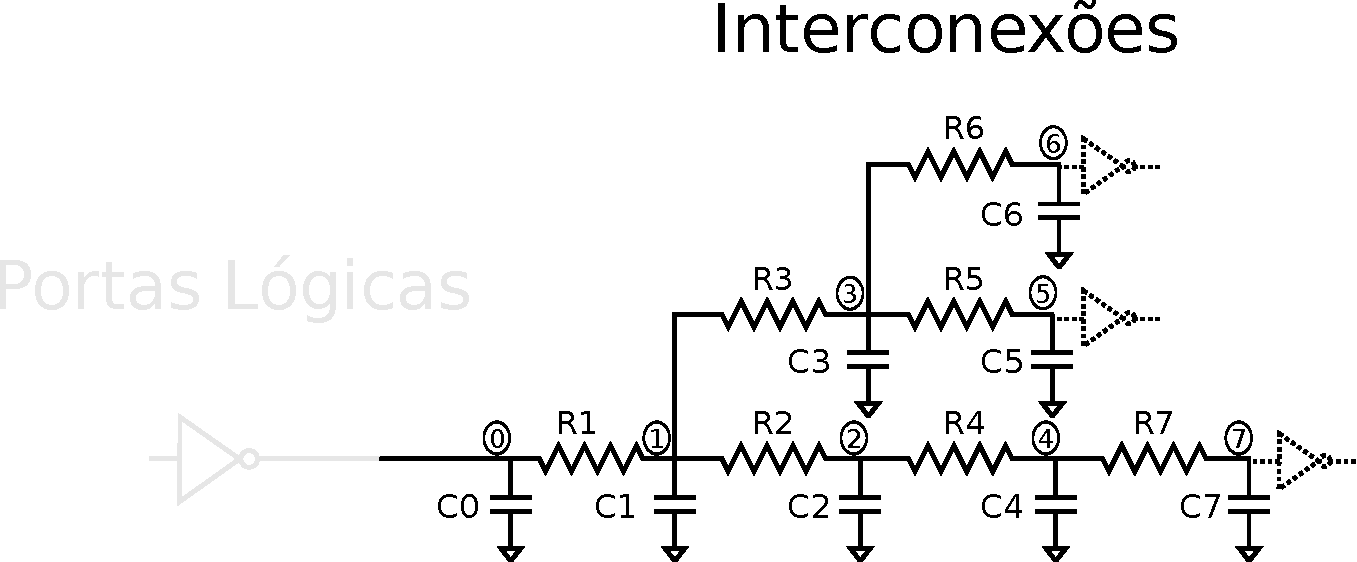
\includegraphics[width=\textwidth]{img/circuito_interconexao.pdf} 
			\end{frame}
			
			\subsubsection*{Modelos de Interconexões}
				\begin{frame}
					\frametitle{Modelo RC Distribuído}
					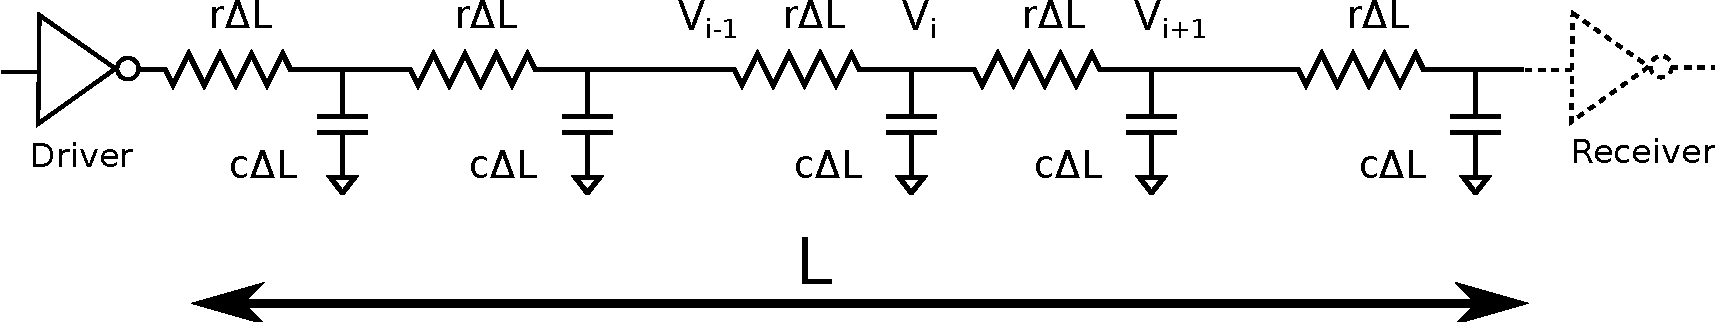
\includegraphics[width=\textwidth]{img/distributed_rc.pdf} 
				\end{frame}
				
				\begin{frame}
					\frametitle{Modelo de Capacitância Concetrada}
					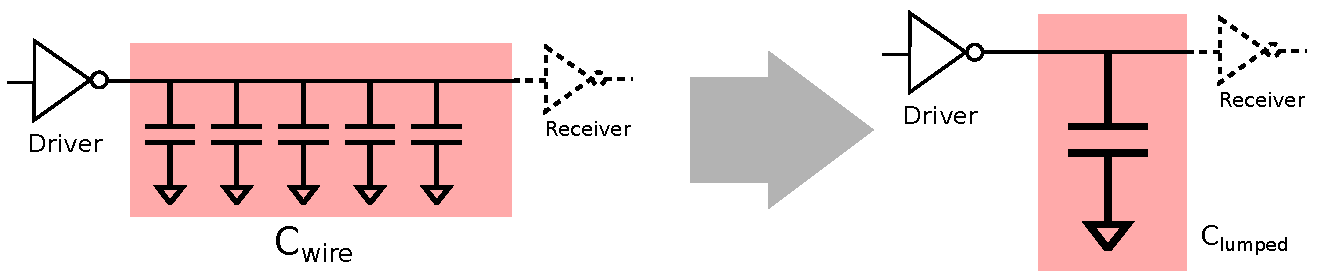
\includegraphics[width=\textwidth]{img/lumped_c.pdf} 
				\end{frame}
				
				\begin{frame}
					\frametitle{Modelo de RC Concentrado}
					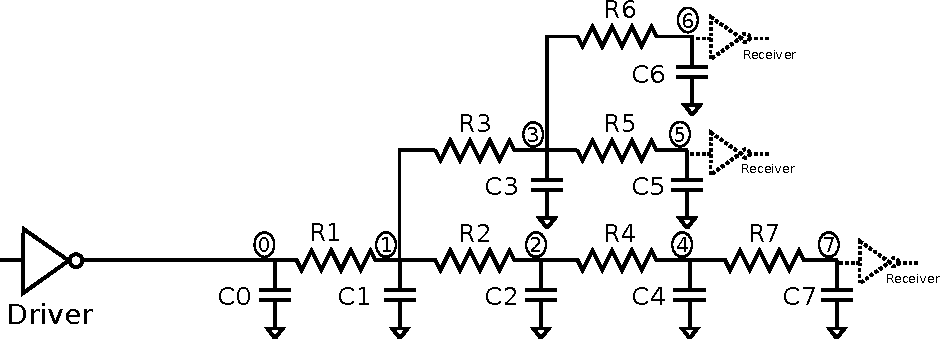
\includegraphics[width=\textwidth]{img/lumped_rc.pdf} 
				\end{frame}
			
			\subsubsection*{Características Temporais}
			\begin{frame}
				\frametitle{Características Temporais}
			\end{frame}
	
	\section{Revisão Bibliográfica}
	
		\begin{frame}
		revs~ao
		\end{frame}
	
	\section{Técnica}
	
		\begin{frame}
		tecnica
		\end{frame}
	
	\section{Análise de Timing Estática}
	
		\begin{frame}
		sta sta
		\end{frame}
	
	\section{Experimentos}
	
		\begin{frame}
		experimentos
		\end{frame}
	
	\section{Conclusões}
	
		\begin{frame}
		conclus~oes
		\end{frame}
	
	\section{Trabalhos Futuros}
		
		\begin{frame}
		trabalhos
		\end{frame}
	
\end{document}
